
\subsection{Mission Study, and Management Plan  }
\label{sec:management}

\vspace{-0.05in}


There are compelling science targets for an imager-based and for 
a spectrometer-based CMB Probe. Our study will investigate the science and technical trade-offs 
for both of these options, and for a combined mission. 

The study itself is open for the entire CMB community and already includes more than 40 scientists representing 
hundreds of years of experience with CMB theory, data analysis, and measurements on all platforms, including satellite missions
that have already flown (WMAP, and \planck ) and the two proposed (LiteBIRD and CORE). 
Figure~\ref{fig:management} shows the management structure of the collaboration. The PI Hanany (who has more 
than 20 years of CMB ballooning experience, co-led MAXIMA and Archeops, was the PI of MAXIPOL and EBEX, and 
is a member of the CORE steering group) 
is advised by a Steering Committee (Bennett, Dodelson, and Page), and assisted by a business office at the University 
of Minnesota.  An Executive Committee (EC) is in charge of the daily operation of the collaboration. The PI and each member of the 
EC also have responsibility for a particular study working group, as outlined in the Figure. Significant overlap and feedback is 
expected among the working groups. 

%and as outlined in more detail below? 
NASA/JPL, lead by CoI Lawrence (Chief Scientist 
at JPL and US \planck\ team lead), will assist with mission design. The PI will lead the study of the Imager and will interface with 
the JPL team. Al Kogut (PI of the Explorer-proposed PIXIE) will lead the spectrometer study. Knox and Flauger will lead the theory and 
foregrounds aspects of the study; McMahon and Lee (PI of the US LiteBIRD team) will lead the study of relevant technologies.  

\begin{figure}[ht!]
\begin{center}
\includegraphics[width=3.2in]{../OrgChart_Names}
%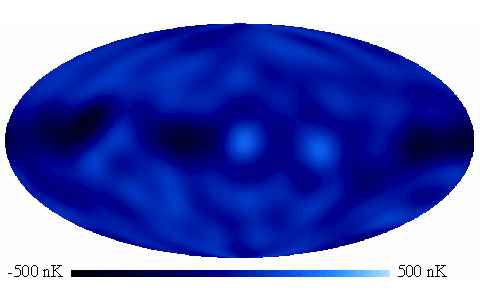
\includegraphics[width=3.2in]{Figures/P353_N_2_12.pdf}
\end{center}
\caption{{\it Left panel:} Contribution to the Stokes $Q$ parameter
  from inflationary $B$-modes for $\ell<12$ and $r=0.001$. {\it Right
    panel:} Noise in the $Planck$ 353 GHz map of the Stokes $Q$
  parameter for $\ell<12$ rescaled to 150\,GHz assuming the spectral
  properties of dust.}
\label{fig:Qrp001}
\end{figure}

The study will be carried out through intra-theme and inter-theme teleconferences; mission design teleconference with JPL engineers; 
mission design meetings at JPL; and a community workshop that is described in more detail below under the the `Space / Sub-Orbital 
Synergy' Theme. 

$\bullet$ \bf{Theory (Knox)} \hspace{0.1in} This working group will survey, summarize, and prioritize the set of 
science goals for the Probe.  Given input on target frequency bands and instrument noise levels the group will 
generate forecasts for the impact of the Probe's products and their ultimate 
significance for physics and astrophysics.

$\bullet$ \bf{Mission (Hanany) and connection with JPL (Lawrence)} \hspace{0.1in} The Mission working group is responsible 
for defining the overall mission 
architecture including telescope implementation, cooling, telemetry, mass, power, and cost. The working group will work closely 
with the JPL lead scientist and JPL mission engineers. \\

$\bullet$ \bf{Imager (Hanany) and Spectrometer (Kogut)} \hspace{0.1in} The imager and spectrometer working groups will 
translate the science goals to 
mission requirements and to a set of optional designs. The designs will include telescopes of various configurations, 
focal planes with several candidate detector technologies and readout schemes. These groups will similarly consider 
the options for spectrometers.  Both groups will work closely 
with the mission working group and with the JPL team to assess the relative merits 
of the optional designs, which will include an imager-only and spectrometer-only options, as well as a combined
instrument.  \\

$\bullet$ \bf{Space / Sub-Orbital Synergy (Jones, Devlin)} \hspace{0.1in} By the time the \ac{CMB} probe is likely to fly,
significant advances are expected to be made on the ground. This is true regardless of the state of the proposed CMB-S4
effort, and even more so should funding for S4 becomes available soon. This working group will assess and recommend the 
most appropriate design parameters such that the data sets from the Probe and sub-orbital measurements complement each other. 
Pertinent questions include: to what extent should the aperture size of the Imaging Probe rely on delensing capabilities provided by 
high resolution measurements from the ground? What is the optimal resolution of a space based mission from the point 
of view of providing foreground subtraction capabilities to sub-orbital missions? What is an optimal overlap in $\ell$-space
coverage? Does the design of a spectrometer depend on the specifics of data available from sub-orbital measurements? 

We are planning a community workshop to address these question, including forming a community consensus on the 
question of the need for a space mission if CMB-S4 is funded. 

$\bullet$ \bf {Complementarity with Other Data Sets (Pryke)} \hspace{0.1in}
The full sky nature, the broad frequency coverage, and the high sensitivity of the CMB-Probe will generate legacy 
data set surpassing that of \planck 's. This working group will survey the possible cross-correlations with astrophysical 
data available at other wavelengths. It will assess whether such cross-correlations can benefit by preferring 
some mission parameter values over others. Examples include adjusting the resolution, and frequency coverage. 
The group will also survey possible sources of systematic uncertainties and how these can be addressed during mission 
design, implementation, and data analysis. 

$\bullet$ \bf {Systematics (Crill)} \hspace{0.1in}

$\bullet$ \bf {Foregrounds (Flauger) } \hspace{0.1in}

$\bullet$ \bf {Technology (Lee, McMahon)} \hspace{0.1in}


Sub-orbital measurements are complementary to those made aboard a space probe. By the time the \ac{CMB} probe is likely to fly significant advances are expected to be made on the ground. 

